%% This is file `medima-template.tex',
%% 
%% Copyright 2018 Elsevier Ltd
%% 
%% This file is part of the 'Elsarticle Bundle'.
%% ---------------------------------------------
%% 
%% It may be distributed under the conditions of the LaTeX Project Public
%% License, either version 1.2 of this license or (at your option) any
%% later version.  The latest version of this license is in
%%    http://www.latex-project.org/lppl.txt
%% and version 1.2 or later is part of all distributions of LaTeX
%% version 1999/12/01 or later.
%% 
%% The list of all files belonging to the 'Elsarticle Bundle' is
%% given in the file `manifest.txt'.
%% 
%% Template article for Elsevier's document class `elsarticle'
%% with harvard style bibliographic references
%%
%% $Id: medima-template.tex 153 2018-12-01 11:38:32Z rishi $
%% $URL: http://lenova.river-valley.com/svn/elsarticle/trunk/medima-template.tex $
%%
%% Use the option review to obtain double line spacing
%\documentclass[times,review,preprint,authoryear]{elsarticle}

%% Use the options 'twocolumn,final' to obtain the final layout
%% Use longtitle option to break abstract to multiple pages if overfull.
%% For Review pdf (With double line spacing)
%\documentclass[times,twocolumn,review]{elsarticle}
%% For abstracts longer than one page.
%\documentclass[times,twocolumn,review,longtitle]{elsarticle}
%% For Review pdf without preprint line
%\documentclass[times,twocolumn,review,nopreprintline]{elsarticle}
%% Final pdf
\documentclass[times,twocolumn,final]{elsarticle}
%%
%\documentclass[times,twocolumn,final,longtitle]{elsarticle}
%%


%% Stylefile to load MEDIMA template
\usepackage{medima}
\usepackage{framed,multirow}
\graphicspath{{./}{../templates/MEDIMA-template/}}
%% The amssymb package provides various useful mathematical symbols
\usepackage{amssymb}
\usepackage{latexsym}

% Following three lines are needed for this document.
% If you are not loading colors or url, then these are
% not required.
\usepackage{url}
\usepackage{xcolor}
\usepackage{graphicx}

\usepackage{hyperref}

\definecolor{newcolor}{rgb}{.8,.349,.1}

\journal{Medical Image Analysis}





% \usepackage{showframe} % for debugging
\newcommand{\carl}[1]{\textcolor{orange}{[Carl: #1]}}
\newcommand{\aleksandar}[1]{\textcolor{cyan}{[Aleksandar: #1]}}
\newcommand{\james}[1]{\textcolor{red}{[James: #1]}}
\definecolor{ForestGreen}{RGB}{34,139,34}
\newcommand{\suggestion}[3]{\textcolor{ForestGreen}{[\textbf{Suggestion (#1):} '\sout{#2}' $\rightarrow$ '#3']}}




\begin{document}

\verso{Given-name Surname \textit{et~al.}}

\begin{frontmatter}

\title{Spatial Analysis for SR$\mu$CT Segmentation}%

\author[1]{James \snm{Avery}\corref{cor1}}
\cortext[cor1]{Corresponding author: 
  Tel.: +45-30229111;  }
\author[3]{Aleksandar \snm{Topic}\fnref{fn1}}
\fntext[fn1]{This is author footnote for second author.}
\author[1]{Carl \snm{Johnsen}}
%% Third author's email
\ead{author3@author.com}
\author[4]{Else \snm{Pinholt}}
\author{Muligvis anden rækkefølge}

\address[1]{University of Copenhagen, Department of Computer Science}
\address[2]{University of Copenhagen, Niels Bohr Institute}
\address[3]{Qtechnology A/S}
\address[4]{University of Southern Denmark}

\received{29 June 2022}
%\finalform{10 May 2013}
%\accepted{13 May 2013}
%\availableonline{15 May 2013}
%\communicated{S. Sarkar}


\begin{abstract}
%%%
Please Type your abstract here. Type your abstract here. Type your abstract
here. Type your abstract here. Type your abstract here. Type your
abstract here. Type your abstract here. Type your abstract here. Type
your abstract here. Type your abstract here. Type your abstract here.
Type your abstract here. Type your abstract here.Type your abstract here. 
Type your abstract here. Type your abstract here. Type your abstract here. 
Type your abstract here. Type your abstract here. Type your abstract here.

Please Type your abstract here. Type your abstract here. Type your abstract
Please Type your abstract here. Type your abstract here. Type your abstract
here. Type your abstract here. Type your abstract here. Type your
abstract here. Type your abstract here. Type your abstract here. Type
your abstract here. Type your abstract here. Type your abstract here.
Type your abstract here. Type your abstract here.
Please Type your abstract here. Type your abstract here. 
Type your abstract here.
%%%%
\end{abstract}

\begin{keyword}
%% MSC codes here, in the form: \MSC code \sep code
%% or \MSC[2008] code \sep code (2000 is the default)
\MSC 41A05\sep 41A10\sep 65D05\sep 65D17
%% Keywords
\KWD Keyword1\sep Keyword2\sep Keyword3
\end{keyword}

\end{frontmatter}

%\linenumbers

\newpage

\section*{Motivation}

 - Hvad er det vi undersøger?
    - Overordnet: Imlantanter i knogler
       - Vil gerne kunne analysere og evaluere kvaliteten af "growth" omkring implantatet
         for at kunne vurdere den underlæggende sundhed og success af operationen
       - Vil gerne kunne afkorte tiden fra operation til analyse til evaluering, samtidigt
         med at kvaliteten af data er stabil til at der er højt evidensgrundlag
       - kunne sige noget om knoglekvaliteten og kompositionen (tæthed, radius, ...)
       - kontakt til implantat: dækket af knogle, blod (forbundet til blodnetværk)
         
 - Hvilke problemer indebærer det som skal løses?
    - Segmentation is hard and time-consuming to do on this type of data.
      - contains noise that is hard to avoid from data acquisition
      - often segmentation is done manually, so being able to automate this data is of great value for the field.
      - Want to avoid using deep learning methods, but keep full transparency 
      - Simpler mathematical methods can be implemented efficiently and consistently

 - Hvordan vil vi bære os ad med at løse problemerne?
    - Det er en forudsætning at vi tydeligt kan observere hvad der sker i bone-to-implant interfacet
    - Den utrolig høje opløsning og kvaliteten af billeder fra SR-micro-CT vil give adgang til
      analyse og segmentering med høj nøjagtighed.
    - Using the geometrical distributions and domain specific knowledge means that we know
      what to expect from the segmentation around all regions.

\subsection*{Data}

\subsubsection*{The physical samples}

The physical samples are prepared for SR$\mu$CT scanning by cutting out a portion of a larger
12mm cylindrical sample. \aleksandar{Better to give a brief chronological tour of how the sample has been handled? Time scale also matters to mention in regards to growth.} The cut samples are 6.5mm cubes \aleksandar{more accurate measures?}. This contains the titanium dental implant (Astra Tech OsseoSpeed, ST Molndal, Sweden), which is 3.5mm in diameter and 8mm long. Along its length the lower 5.5mm has larger threads and is attached to recipient bone. The upper 2.5mm has smaller threads and is where newly formed bone is to be assessed. Sorrounding the bone and implant contact-region are cavities containing resin, air, blood vessels and other fibrous tissue. This is shown in figure \ref{fig:3viewsample}.


\begin{figure}%[!t]
\centering
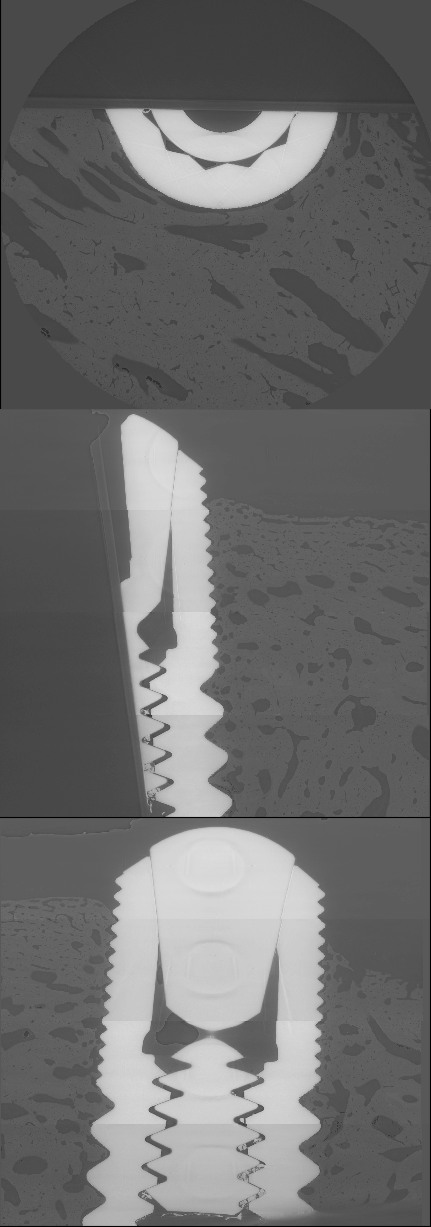
\includegraphics[scale=0.50]{figures/3_view_sample.png}
\caption{\aleksandar{Temporary example figure of sample in x,y,z dimension. It could perhaps even be manually annotated (meaning we can indicate roughly what regions correspond to: resin, air, implant, bone), and related to the physical scale mentioned above? Maybe as simple as overlaying a ruler with the given scale?}}
\label{fig:3viewsample}
\end{figure}

Each material has a different density and thus absorption. The titanium implant has higher absorption than bone.
Bone material then has higher absorption than its sorrounding tissue, vessels, air and resin.

\subsubsection*{Data acquisition}

It can be difficult to study and evaluate the bone structure and blood network without destroying or
manipulating the sample. X-ray computed tomography is a widely used tool for non-intrusive medical
imaging. By exposing a subject to X-rays, we can map the linear attentuation coffecient of the passing
rays. Each ray is attenuated relatively to the density and composition of the material it passes. By
rotating either the scanner or the sample we can get a full 3D image representation of the inner
structure of the sample. Each volumetric pixel (voxel) then represents the X-ray attenuation at its spatial position. We can therefore reliably use X-rays to internally characterise samples in a non-intrusive and non-destructive manner. Regular CT-scans can provide spatial resolutions on the order of millimetre scale.\aleksandar{ref} The more modern micro computed tomography ($\mu$CT) can provide much higher spatial resolution on the micrometre scale.\aleksandar{ref} Both setups utilize poly-energetic beams, which can cause artifacts around high density regions. This effect is called beam-hardening\aleksandar{ref}, and occurs when rays with lower energy are attenuated more frequently. This offsets the local contrast, by overestimating the attenuation, leaving lighter spots on the image. Many other types of artifacts will also occur in these common scanners, but most is taken into account by calibration using phantoms and pre-hardening the beam before it reaches the sample. Due to its common usage, much software also exists to correct for noise and smaller imperfections during reconstruction\aleksandar{ref}.

This work focuses on data acquired by Synchrotron Radiation micro-CT (SR$\mu$CT). For this imaging
technique, electrons are accelerated to ultra-relativistic speeds in trajectories directed by strong
magnetic fields. Contrary to both CT and $\mu$CT, this approach requires a large particle accelerator, and is not standard medical or laboratory equipment\aleksandar{ref}. The added complexity means that SR$\mu$CT can offer an even better spatial resolution of up to 0.1 $\mu$m. The resulting beams are high in brilliance and collimation which gives a very clear signal. Its mono-energetic nature also means that images are not subject to artifacts from beam-hardening.

\aleksandar{Can we confirm whether data was acquired at the ESRF and at which beamline? Also which energies were used? All this could be important for reproducibility.}

\aleksandar{Was filtered backprojection used to do reconstruction, and who has done that? Was it done at ESRF?}

\subsubsection*{Image data}

A single image sample contains voxels with of spatial resolution 1.875$\mu$m. The physical size of
a sample is about 6.5mm, which makes the raw dimensions of a single image $(3480,3480,3384)$ pixels.
For computational purposes, this has been cropped to be divisible by $2^5=32$. A full image sample
is further split into 4-6 sub-volumes through the height of the implant. This gives a size of $(3456,3456,810)$ pixels per sub-volume, where the last axis gets stacked for a full volume.

\aleksandar{OBS: 846 i rå størelse, 810 er efter volume-matching.}

\aleksandar{Important to explain a bit about how the samples were cut during acquisition. How were the samples secured in order not to be shifted too much etc.}

\section*{Physical effects, noise and artifacts}

Noise in tomography is unavoidable, and it makes segmentation harder. Matarials may be well separated from certain angles in the 3d-reconstructed image, but overlap from others. Some noise like that corrected by flat-field correction is very uniformly distributed across images. Some noise is however very spatially dependent on its sorrounding regions. Since we know the compositions of the materials being imaged, we can counter some of these effects during segmentation. The noise effects manifest themselves as numerical shifts in voxel-values as a function of their position. This is a direct result of a misrepresented attenuation along the axis the X-rays are passing. 

\aleksandar{perhaps we should mention at what energies the data is taken. This helps to narrow which types of effects play into the data.}

Low energy rays contribute mostly with noise from scattering effects. A ray will propagate through a material, get scattered and diffract from its initial trajectory. This gives a misrepresentation of the attenuation along its initial trajectory.

Streaking artifacts from dense implant region, but also in the transition from bone to softer tissue.

...

For SR$\mu$CT a high photon flux allows for very short exposure times \citep{srexptime}.
This can help counter noise from suboptimal counting statistics\citep{srnoise}.


* Gå fra brede effekter som viser sig i hele billedet (og er mere generelle) -> Til de mere specifikke effekter som er mere specifikke for vores case

* genskær fra voxels
mørke effekter modsat lysere effekter fra beam-hardening (x-rays er inverteret)

Forklare hvorfor vi ser mørke områder, særligt at det mørke lægger sig omkring implantatet,
men at det så aftager mod knoglen, for så at blive kraftigere og bredere helt ved knoglen..
nok refraktion osv. \aleksandar{OBS: before talking about specific noise in our data, we should probably include one or more examples of noise that shows how the segmentation is made harder due to this noise.}


\section*{Solutions}

\aleksandar{Work-in-progress}

Individual materials are segmented from the full image, which is represented by their respective histograms.

\begin{equation}
H(x,v) = \sum_{m=1}^{n} g_{m}(x,v) + r(x,v)
\end{equation}

Where $g_m$ represents a histogram for materials $m\in\{1,n\}$, and $r(x,v)$ is incorrectly identified remainding region.

We find the probability for a certain material as:

\begin{equation}
p(m|x,v) = \frac{g_{m}(x,v)}{H(x,v)}
\end{equation}

We then have a single distribution is given by a piecewise polynomial:

\begin{equation}
g_{m}(x,v) = a_{m}(x) e^{ -b_{m}(x) |v-c_{m}(x)|^{d_{m}(x)} }
\end{equation}

Where a is the height, b is the width, c is the centre and d is the exponent.

If we were to look at the distributions for individual slices, we would get too much variance.
Instead we would like to fit the individual coefficients to get a smooth function.

\subsection*{Miscellaneous}

We shall go through these subjects and explain what was done and how + why. We briefly explain how the method works.

\begin{itemize}
 \item Volume matching
 \item Find implant mask
 \item EDT (Euclidean distance transform)
 \item Gauss
 \item Gauss + EDT
 \item Hist(x,y,z,r)
 \item Find lines / ridges
 \item Get distributions
 \item Beskrive processen under GUI trinvist
 \item Segment materials from distributions
 \item Bayesian combination of materials from their distributions
\end{itemize}

\subsection*{Probabilities}

\aleksandar{Work-in-progress}

Ud fra et 3d-billede (volumen), kan vi tælle os til de enkelte fordelinger

p(I), p(I|x), p(I|y), p(I|z), p(I|r), hvor $r=\sqrt{(x-x_0)^2+(y-y_0)^2}$

ved at finde peaks og fitte distributioner kan vi da finde approksimationer til

p(c|I), p(c|I,x), p(c|I,y), p(c|I,z), p(c|I,r)

hvor c er klasserne, fx knogle, blodåre, væv, ... 

Vi vil gerne finde kombinationsfordelinger som kan klassificere voxels ved brug af mere information end kun intensiteten - blandt andet hvor voxelen befinder sig.

Ud fra fx p(c|I,x) og p(c|I,y) og ... vil vi gerne approksimere p(c|I,x,y,z,r) uden at skulle repræsentere den eksplicit som et kæmpe volumen.

Dette vil vi gøre ved at bruge betinget uafhængiged. \aleksandar{Evt inkludere bevis for at det er validt. Ellers så blot forklare hvordan sandsynlighederne sammensættes og bruges.}

% ------------------------------------------ %
% Underneath this is Elseviers template text %
% ------------------------------------------ %

%% main text
\section{Note}
\label{sec1}
Please use \verb+elsarticle.cls+ for typesetting your paper.
Additionally load the package \verb+medima.sty+ in the preamble using
the following command: 
\begin{verbatim} 
  \usepackage{medima}
\end{verbatim}

Following commands are defined for this journal which are not in
\verb+elsarticle.cls+. 
\begin{verbatim}
  \received{}
  \finalform{}
  \accepted{}
  \availableonline{}
  \communicated{}
\end{verbatim}

Any instructions relavant to the \verb+elsarticle.cls+ are applicable
here as well. See the online instruction available on:
\makeatletter
\if@twocolumn
\begin{verbatim}
 http://support.stmdocs.com/wiki/
 index.php?title=Elsarticle.cls
\end{verbatim}
\else
\begin{verbatim}
 http://support.stmdocs.com/wiki/index.php?title=Elsarticle.cls
\end{verbatim}
\fi

\subsection{Entering text}
\textcolor{newcolor}{\bf There is no page limit.}

\section{The first page}
Avoid using abbreviations in the title. Next, list all authors with
their first names or initials and surnames (in that order). Indicate
the author for correspondence (see elsarticle documentation).

Present addresses can be inserted as footnotes. After having listed all
authors' names, you should list their respective affiliations. Link
authors and affiliations using superscript lower case letters.

\subsection{The Abstract}
An Abstract is required for every paper; it should succinctly summarize
the reason for the work, the main findings, and the conclusions of the
study. The abstract should be no longer than 200 words. Do not include
artwork, tables, elaborate equations or references to other parts of
the paper or to the reference listing at the end. ``Comment'' papers
are exceptions, where the commented paper should be referenced in full
in the Abstract.

The reason is that the Abstract should be understandable in itself to
be suitable for storage in textual information retrieval systems.

\textit{Example of an abstract: A biometric sample collected in an
uncontrolled outdoor environment varies significantly from its
indoor version. Sample variations due to outdoor environmental
conditions degrade the performance of biometric systems that
otherwise perform well with indoor samples. In this study, we
quantitatively evaluate such performance degradation in the case
of a face and a voice biometric system. We also investigate how
elementary combination schemes involving min-max or z
normalization followed by the sum or max fusion rule can
improve performance of the multi-biometric system. We use
commercial biometric systems to collect face and voice samples
from the same subjects in an environment that closely mimics the
operational scenario. This realistic evaluation on a dataset of
116 subjects shows that the system performance degrades in
outdoor scenarios but by multimodal score fusion the
performance is enhanced by 20\%. We also find that max rule
fusion performs better than sum rule fusion on this dataset. More
interestingly, we see that by using multiple samples of the same
biometric modality, the performance of a unimodal system can
approach that of a multimodal system.}

\section{The main text}

Please divide your article into (numbered) sections (You can find the
information about the sections at
\url{http://www.elsevier.com/wps/find/journaldescription.cws_home/505619/authorinstructions}).
Ensure that all tables, figures and schemes are cited in the text in
numerical order. Trade names should have an initial capital letter, and
trademark protection should be acknowledged in the standard fashion,
using the superscripted characters for trademarks and registered
trademarks respectively. All measurements and data should be given in
SI units where possible, or other internationally accepted units.
Abbreviations should be used consistently throughout the text, and all
nonstandard abbreviations should be defined on first usage
[removed].

\begin{table*}[!t]
\caption{\label{tab1}Summary of different works pertaining to face and
speech fusion}
\centering
\begin{tabular}{|p{2.25cm}|p{2cm}|l|p{4cm}|p{3cm}|p{2cm}|}
\hline
Study & Algorithm used & DB Size & Covariates of interest & 
Top individual performance & Fusion\newline Performance\\
\hline
UK-BWG
(Mansfield et al.,
2001) &
Face, voice:\newline
Commercial & 200 & Time: 1--2 month\newline
separation (indoor) & 
TAR$^*$ at 1\% FAR$^{\#}$\newline
Face: 96.5\%\newline
Voice: 96\%
& --\\
\hline
Brunelli
(Brunelli and
Falavigna, 1995) & 
Face:\newline
Hierarchical\newline
correlation\newline
Voice:\newline
MFCC & 
87 & 
Time: 3 sessions, time\newline
unknown (indoor) & 
Face:\newline
TAR = 92\% at\newline
4.5\% FAR\newline
Voice:\newline
TAR = 63\% at\newline
15\% FAR
&
TAR =98.5\%\newline
at 0.5\% FAR\\
\hline
Jain
(Jain et al., 1999)
&
Face:\newline
Eigenface\newline
Voice:\newline
Cepstrum\newline
Coeff. Based
&
50
&
Time: Two weeks (indoor)
&
TAR at 1\% FAR\newline
Face: 43\%\newline
Voice: 96.5\%\newline
Fingerprint: 96\%
& 
Face $+$ Voice $+$\newline
Fingerprint $=$\newline
98.5\%\\
\hline
Sanderson
(Sanderson and
Paliwal, 2002)
&
Face: PCA\newline
Voice: MFCC &
43 
& Time: 3 sessions (indoor)\newline
Noise addition to voice & 
Equal Error Rate\newline
Face: 10\%\newline
Voice: 12.41\%
&
Equal Error\newline
Rate 2.86\% \\
\hline
Proposed study & 
Face, voice:\newline
Commercial & 116 &
Location: Indoor and\newline
Outdoor (same day)\newline
Noise addition to eye\newline 
coordinates 
&
TARs at 1\% FAR\newline
Indoor-Outdoor\newline
Face: 80\%\newline
Voice: 67.5\%
&
TAR = 98\%\newline
at 1\% FAR\\
\hline
\multicolumn{6}{@{}l}{$^*$TAR--True Acceptance Rate\qquad 
$^{\#}$ FAR--False Acceptance Rate}
\end{tabular}
\end{table*}


\subsection{Tables, figures and schemes}
Graphics and tables may be positioned as they should appear in the
final manuscript. Figures, Schemes, and Tables should be numbered.
Structures in schemes should also be numbered consecutively, for ease
of discussion and reference in the text. \textcolor{newcolor}{\bf
Figures should be maximum half a page size.}

Depending on the
amount of detail, you can choose to display artwork in one column (20
pica wide) or across the page (42 pica wide). Scale your artwork in
your graphics program before incorporating it in your text. If the
artwork turns out to be too large or too small, resize it again in your
graphics program and re-import it. The text should not run along the
sides of any figure. This is an example for citation [removed].

\begin{figure}[!t]
\centering
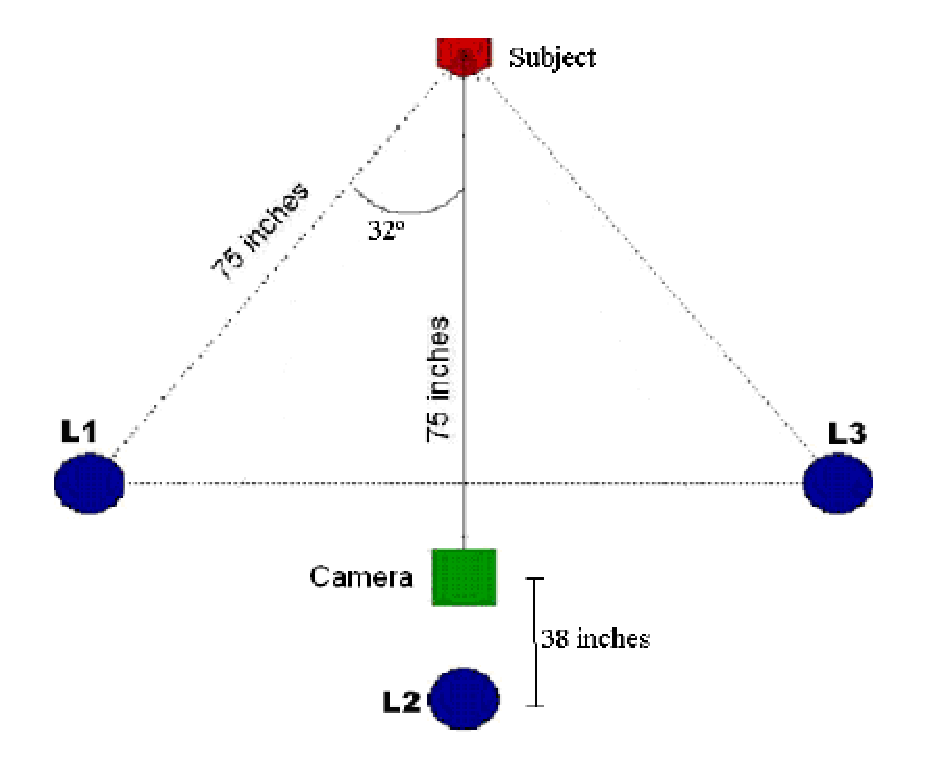
\includegraphics[scale=.5]{medimafig01}
\caption{Studio setup for capturing face images indoor. Three light
sources L1, L2, L3 were used in conjunction with normal office lights.}
\end{figure}

You might find positioning your artwork within the text difficult
anyway. In that case you may choose to place all artwork at the end of
the text and insert a marker in the text at the desired place. In any
case, please keep in mind that the placement of artwork may vary
somewhat in relation to the page lay-out [removed].

This can easily be achieved using \verb+endfloat.sty+ package. Please
refer the following documentation to use this package.
\makeatletter
\if@twocolumn
\begin{verbatim}
  http://mirrors.ctan.org/macros/latex/contrib/
  endfloat/endfloat.pdf
\end{verbatim}
\else
\begin{verbatim}
  http://mirrors.ctan.org/macros/latex/contrib/endfloat/endfloat.pdf
\end{verbatim}
\fi
\makeatother

\textcolor{newcolor}{\bf You should insert a caption for the figures
below the figures and for the tables the caption should be above the
tables.} 

Please remember that we will always also need highresolution versions
of your artwork for printing, submitted as separate files in standard
format (i.e. TIFF or EPS), not included in the text document. Before
preparing your artwork, please take a look at our Web page:
\url{http://www.elsevier.com/locate/authorartwork}.


\subsection{Lists}

For tabular summations that do not deserve to be presented as
a table, lists are often used. Lists may be either numbered or
bulleted. Below you see examples of both.
\begin{enumerate}
\item The first entry in this list
\item The second entry
\begin{enumerate}
\item A subentry
\end{enumerate}
\item The last entry
\end{enumerate}
\begin{itemize}
\item A bulleted list item
\item Another one
\end{itemize}

\subsection{Equations}
Conventionally, in mathematical equations, variables and
anything that represents a value appear in italics.
All equations should be numbered for easy referencing. The number
should appear at the right margin.
\begin{equation}
S_{\rm pg}'=\frac{S_{\rm pg}-\min(S_{\rm pG})}
 {\max(S_{\rm pG}-\min(S_{\rm pG})}
\end{equation}
In mathematical expressions in running text ``/'' should be used for
division (not a horizontal line). 

\section*{Acknowledgments}
Acknowledgments should be inserted at the end of the paper, before the
references, not as a footnote to the title. Use the unnumbered
Acknowledgements Head style for the Acknowledgments heading.

\section*{References}

Please ensure that every reference cited in the text is also present in
the reference list (and vice versa).

\section*{\itshape Reference style}

Text: All citations in the text should refer to:
\begin{enumerate}
\item Single author: the author's name (without initials, unless there
is ambiguity) and the year of publication;
\item Two authors: both authors' names and the year of publication;
\item Three or more authors: first author's name followed by `et al.'
and the year of publication.
\end{enumerate}
Citations may be made directly (or parenthetically). Groups of
references should be listed first alphabetically, then chronologically.

%%Harvard
\bibliographystyle{model2-names.bst}\biboptions{authoryear}
\bibliography{refs}

\section*{Supplementary Material}

Supplementary material that may be helpful in the review process should
be prepared and provided as a separate electronic file. That file can
then be transformed into PDF format and submitted along with the
manuscript and graphic files to the appropriate editorial office.

\end{document}

%%
